\subsection{特例:周期函数的傅里叶级数}

\begin{remark}
    周期信号通常可以被表示为
    \begin{align*}
        f(t) = \sum_{n = -\infty}^{\infty} f_0(t - nT),
    \end{align*}
    其中 $f_0(t)$ 是一个周期为 $T$ 的函数。
\end{remark}

\subsubsection{周期函数的正交分解}

\begin{definition}[狄义赫利条件]
    设有一信号 $f(t)$,若它满足以下条件:
    \begin{enumerate}[label=(\arabic*)]
        \item $f(t)$ 间断点的个数有限,
        \item $f(t)$ 极值点的个数有限,
        \item $f(t)$ 绝对积分数值有限,
    \end{enumerate}
    则称 $f(t)$ 满足\bd{狄义赫利条件}。
\end{definition}

\begin{theorem}
    满足狄义赫利条件的\bd{周期函数}
    都可以在一组\bd{完备的正交基函数}上展开成为\bd{无穷级数}。
\end{theorem}

\begin{definition}[傅里叶级数展开]
    如果完备的正交函数集是三角函数集或指数函数集,
    则周期函数展成的级数就是\bd{傅里叶级数}。
    相应的级数通常被称为\bd{三角形式傅里叶级数}和\bd{指数形式傅里叶级数}。
\end{definition}

\begin{note}
    回忆三角函数集和指数函数集的定义:
    \begin{itemize}
        \item 三角函数集(不完备):$\{1, \cos(\omega_0t + \varphi_1), \cos(2\omega_0t + \varphi_2), \cdots, \cos(n\omega_0 t + \varphi_n)\}$,
            即 $\{1, \cos(n\omega_0t), \sin(n\omega_0t)\}$,其中 $n$ 取遍 $\set{N}^{+}$。
        \item 三角函数集(完备):$\{1, \cos(n\omega_0 t), \sin(n\omega_0 t)\}$,其中 $n$ 取遍 $\set{N}^{+}$。
        \item 指数函数集:$\{\mathe^{\mathi n\omega_0t} \mid n \in \set{Z}\}$。
    \end{itemize}
    请注意,三角函数集中的 $n$ 是\bd{正整数},而指数函数集中的 $n$ 是\bd{整数}。
\end{note}

\begin{definition}[三角形式傅里叶级数]
    设周期函数 $f(t)$ 的周期为 $T_0$,令 $\omega_0 = 2\pi/T_0$,
    函数集 $\{1, \cos(n\omega_0 t), \sin(n\omega_0 t)\}$ 是一组完备的正交函数集,
    其中 $n$ 取遍 $\set{N}^{+}$。则 $f(t)$ 可以被展开成三角函数的无穷级数形式:
    \begin{align*}
        f(t) = a_0 + \sum_{n = 1}^{+\infty}(a_n\cos(n\omega_0 t) + b_n\sin(n\omega_0 t)),
    \end{align*}
    系数 $a_n$ 和 $b_n$ 统称为\bd{三角形式的傅里叶级数系数},简称为\bd{傅里叶系数}。
\end{definition}

\begin{lemma}
    设周期函数 $f(t)$ 的周期为 $T_0$,令 $\omega_0 = 2\pi/T_0$,
    函数集 $\{1, \cos(n_0\omega_0 t), \sin(n_0\omega_0 t)\}$ 是一组完备的正交函数集,
    其中 $n$ 取遍 $\set{N}^{+}$。则
    \begin{align*}
        \int_{t_0}^{t_0 + T_0}\cos(m\omega_0 t)\cos (n\omega_0 t)\D{t} & = \begin{cases}
            T_0 / 2, & m = n \neq 0, \\
            T_0, & m = n = 0, \\
            0, & m \neq n.
        \end{cases} \\
        \int_{t_0}^{t_0 + T_0}\sin(m\omega_0 t)\sin (n\omega_0 t)\D{t} & = \begin{cases}
            T_0 / 2, & m = n \neq 0, \\
            0, & \text{otherwise}.
        \end{cases} \\
        \int_{t_0}^{t_0 + T_0}\cos(m\omega_0 t)\sin (n\omega_0 t)\D{t} & = 0.
    \end{align*}
\end{lemma}

\begin{proof}
    首先证明 $\cos(m\omega_0 t)\cos(n\omega_0 t)$ 的积分:
    \begin{align*}
        \int_{t_0}^{t_0 + T_0}\cos(m\omega_0 t)\cos(n\omega_0 t)\D{t}
        & = \frac{1}{2}\int_{t_0}^{t_0 + T_0}\left(\cos((m + n)\omega_0 t) + \cos((m - n)\omega_0 t)\right)\D{t} \\
        & = \begin{cases}
            T_0 / 2, & m = n \neq 0, \\
            T_0, & m = n = 0, \\
            0, & m \neq n.
        \end{cases}
    \end{align*}
    然后证明 $\sin(m\omega_0 t)\sin(n\omega_0 t)$ 的积分:
    \begin{align*}
        \int_{t_0}^{t_0 + T_0}\sin(m\omega_0 t)\sin(n\omega_0 t)\D{t}
        & = \frac{1}{2}\int_{t_0}^{t_0 + T_0}\left(\cos((m - n)\omega_0 t) - \cos((m + n)\omega_0 t)\right)\D{t} \\
        & = \begin{cases}
            T_0 / 2, & m = n \neq 0, \\
            0, & \text{otherwise}.
        \end{cases}
    \end{align*}
    最后证明 $\cos(m\omega_0 t)\sin(n\omega_0 t)$ 的积分:
    \begin{align*}
        \int_{t_0}^{t_0 + T_0}\cos(m\omega_0 t)\sin(n\omega_0 t)\D{t}
        & = \frac{1}{2}\int_{t_0}^{t_0 + T_0}\left(\sin((m + n)\omega_0 t) - \sin((m - n)\omega_0 t)\right)\D{t} \\
        & = 0.
    \end{align*}
    命题得证。
\end{proof}

\begin{corollary}
    傅里叶系数 $a_n$ 和 $b_n$ 的表达式为:
    \begin{align*}
        a_0 & = \frac{1}{T_0}\int_{t_0}^{t_0 + T_0}f(t)\D{t}, \\
        a_n & = \frac{2}{T_0}\int_{t_0}^{t_0 + T_0}f(t)\cos(n\omega_0 t)\D{t}, \\
        b_n & = \frac{2}{T_0}\int_{t_0}^{t_0 + T_0}f(t)\sin(n\omega_0 t)\D{t}.
    \end{align*}
\end{corollary}

\begin{proof}
    已知 $f(t) = a_0 + \sum_{n = 1}^{+\infty}a_n\cos(n\omega_0 t) + b_n\sin(n\omega_0 t)$,则
    等式两边同时在 $[t_0, t_0 + T_0]$ 上积分,有
    \begin{align*}
        \int_{t_0}^{t_0 + T_0}f(t)\D{t} & = \int_{t_0}^{t_0 + T_0}a_0\D{t} + \sum_{n = 1}^{+\infty}\int_{t_0}^{t_0 + T_0}a_n\cos(n\omega_0 t)\D{t} + \sum_{n = 1}^{+\infty}\int_{t_0}^{t_0 + T_0}b_n\sin(n\omega_0 t)\D{t} \\
        & = \int_{t_0}^{t_0 + T_0}a_0\D{t} + \sum_{n = 1}^{+\infty}a_n\int_{t_0}^{t_0 + T_0}\cos(n\omega_0 t)\D{t} + \sum_{n = 1}^{+\infty}b_n\int_{t_0}^{t_0 + T_0}\sin(n\omega_0 t)\D{t} \\
        & = T_0 \cdot a_0 + \sum_{n = 1}^{+\infty}a_n\cdot 0 + \sum_{n = 1}^{+\infty}b_n\cdot 0 \\
        & = T_0 \cdot a_0.
    \end{align*}
    因此,有 $a_0 = \frac{1}{T_0}\int_{t_0}^{t_0 + T_0}f(t)\D{t}$。

    同理,在等式左右两侧乘上 $\cos(n \omega_0 t)$ 之后再在 $[t_0, t_0 + T_0]$ 上积分,
    可得 $a_n = \frac{2}{T_0}\int_{t_0}^{t_0 + T_0}f(t)\cos(n\omega_0 t)\D{t}$。
    在等式左右两侧乘上 $\sin(n \omega_0 t)$ 之后再在 $[t_0, t_0 + T_0]$ 上积分,
    可得可得 $b_n = \frac{2}{T_0}\int_{t_0}^{t_0 + T_0}f(t)\sin(n\omega_0 t)\D{t}$。
    命题得证。
\end{proof}

\begin{remark}
    常用的正交函数集的基本函数,除正弦型函数(含复指数函数)外,
    还有勒让德函数(Legendre function)、贝塞尔函数(Bessel function)、
    沃尔什函数(Walsh function)等,不一一列举。
\end{remark}

\begin{definition}[复指数形式傅里叶级数]
    由欧拉公式可以得到 $\cos(n\omega_0 t) = (\mathe^{\mathi n\omega_0 t} + \mathe^{-\mathi n\omega_0 t}) / 2$,
    以及 $\sin(n\omega_0 t) = (\mathe^{\mathi n\omega_0 t} - \mathe^{-\mathi n\omega_0 t}) / 2\mathi$。
    因此,我们可以将三角函数形式的傅里叶级数改写为:
    \begin{align*}
        f(t) = a_0 + \sum_{i = 1}^{+\infty}\left(\frac{a_n - \mathi b_n}{2}\mathe^{\mathi n\omega_0 t} + \frac{a_n + \mathi b_n}{2}\mathe^{-\mathi n\omega_0 t}\right).
    \end{align*}
    记 $F(\cdot)$ 为一个函数,则 $a_0, a_n, b_n$ 可以看做是 $(n, \omega_0)$ 对应的函数值。则
    \begin{align*}
        f(t) = F(0) + \sum_{i = 1}^{+\infty}\left(F(n\omega_0)+ F(-n\omega_0)\right)
    \end{align*}
    再记 $F_n = F(n\omega_0)$,则可将 $f(t)$ 表示为\bd{复指数形式的傅里叶级数}:
    \begin{align*}
        f(t) = \sum_{n = -\infty}^{+\infty}F_n\mathe^{\mathi n\omega_0 t},
    \end{align*}
    其中 $F_n = (a_n - \mathi b_n) / 2$ 为\bd{复指数形式的傅里叶级数系数}。
\end{definition}

\begin{property}
    复指数形式傅里叶级数的系数 $F_n$ 的表达式为:
    \begin{align*}
        F_n = \frac{1}{T_0}\int_{t_0}^{t_0 + T_0}f(t)\mathe^{-\mathi n\omega_0 t}\D{t}.
    \end{align*}
\end{property}

\begin{proof}
    (方法一)
    \begin{align*}
        F_n & = \frac{a_n - \mathi b_n}{2} \\
        & = \frac{1}{2} \cdot \frac{2}{T_0}\int_{t_0}^{t_0 + T_0}f(t)\cos(n\omega_0 t)\D{t} - \frac{\mathi}{2} \cdot \frac{2}{T_0}\int_{t_0}^{t_0 + T_0}f(t)\sin(n\omega_0 t)\D{t} \\
        & = \frac{1}{T_0}\int_{t_0}^{t_0 + T_0}f(t)(\cos(n\omega_0 t) - \mathi \sin(n\omega_0 t))\D{t} \\
        & = \frac{1}{T_0}\int_{t_0}^{t_0 + T_0}f(t)\mathe^{-\mathi n\omega_0 t}\D{t}.
    \end{align*}
    命题得证。
\end{proof}

\begin{proof}
    (方法二)
    由级数展开的定义,在函数集 $\{\mathe^{\mathi n\omega_0 t}\}$ 上展开,有
    \begin{align*}
        F_n & = \frac{\ip{f}{\varphi_n}}{\ip{\varphi_n}{\varphi_n}}\\
        & = \frac{1}{k_n}\int_{t_0}^{t_0 + T_0}f(t) \mathe^{-\mathi n\omega_0 t}\D{t}.
    \end{align*}
    而 $k_n$ 可以计算如下:
    \begin{align*}
        k_n & = \int_{t_0}^{t_0 + T_0}\mathe^{\mathi n\omega_0 t}\mathe^{-\mathi n\omega_0 t}\D{t} \\
        & = \int_{t_0}^{t_0 + T_0}\D{t} \\
        & = T_0.
    \end{align*}
    因此 $F_n = \frac{1}{T_0}\int_{t_0}^{t_0 + T_0}f(t)\mathe^{-\mathi n\omega_0 t}\D{t}$。
\end{proof}

\begin{property}
    对偶信号序列的傅里叶级数而言,$F_n$ 是偶对称的实数序列,
    对奇信号序列的傅里叶级数而言,$F_n$ 是奇对称的纯虚序列。
\end{property}

\begin{proof}
    考虑关系式 $F_n = (a_n - \mathi b_n) / 2$:
    \begin{itemize}
        \item 对于偶信号序列而言,$a_n \neq 0, b_n = 0$,所以 $F_n$ 只有直流分量和余弦项。
        \item 对于奇信号序列而言,$a_n = 0, b_n \neq 0$,所以 $F_n$ 只有正弦项。
    \end{itemize}
    命题得证。
\end{proof}

\begin{corollary}[帕斯瓦尔定理的推论]
    周期信号的\bd{平均功率}等于傅里叶级数展开各谐波分量有效值的平方和。
    也就是说,\bd{时域和频域的能量守恒}。
\end{corollary}

\begin{proof}
    由帕斯瓦尔定理知,
    \begin{align*}
        \int_{t_0}^{t_0 + T_0}\|f(t)\|^2\D{t} & = \|a_0\|^2\cdot k_0
            + \sum_{i = 1}^{+\infty}\|a_i\|^2k_{\cos, i}
            + \sum_{i = 1}^{+\infty}\|b_i\|^2k_{\sin, i} \\
        & = T_0 \cdot \|a_0\|^2 + \frac{T_0}{2}\cdot \sum_{i = 1}^{+\infty}(\|a_i\|^2 + \|b_i\|^2).
    \end{align*}
    因此,有
    \begin{align*}
        P & = \overline{\|f(t)\|^2} = \frac{1}{T_0}\int_{t_0}^{t_0 + T_0}\|f(t)\|^2\D{t} \\
        & = \frac{1}{T_0}\left(T_0 \cdot \|a_0\|^2 + \frac{T_0}{2}\cdot \sum_{i = 1}^{+\infty}(\|a_i\|^2 + \|b_i\|^2)\right) \\
        & = \|a_0\|^2 + \frac{1}{2}\sum_{i = 1}^{+\infty}(\|a_i\|^2 + \|b_i\|^2) \\
        & = \sum_{i = -\infty}^{+\infty}\|F_n\|^2.
    \end{align*}
    命题得证。
\end{proof}

\subsubsection{周期信号的傅里叶级数}

\begin{definition}
    由于 $F_n \in \set{C}$,所以它谱线并不方便在二维平面上表示,
    因此 $F_n$ 可以从两个角度来表示:一个是 $|F_n|$,即为\bd{幅度谱},
    另一个是 $\varphi_n = \arg(F_n)$,即为\bd{相位谱}。

    周期信号的傅里叶级数可视化如图 \ref{fig:periodic-signal-fourier-series} 所示。
    \begin{figure}[H]
        \centering
        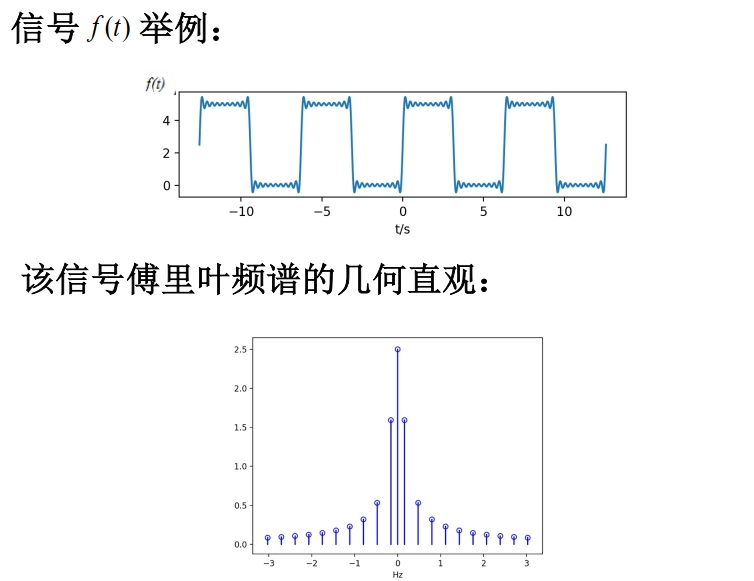
\includegraphics[width = 0.6\textwidth]{chap2/img/periodic-signal-fourier-series.png}
        \caption{周期信号的傅里叶级数}
        \label{fig:periodic-signal-fourier-series}
    \end{figure}
\end{definition}

\begin{property}[周期信号的傅里叶频谱特点]
    周期信号的傅里叶频谱有以下特点:
    \begin{itemize}
        \item 仅在一些离散的频率点 $n\omega_0, n \in \set{Z}$ 上有值。
        \item 离散间隔为 $\omega_0 = 2\pi f_0 = 2\pi / T_0$。
        \item $F_n$ 是双边谱,即 $F_n = F_{-n}$,因此正负频率的频谱幅度相加才是实际幅度。
        \item 信号的功率为 $\sum_{-\infty}^{+\infty}\|F_n\|^2$。
    \end{itemize}
\end{property}

\begin{example}[周期矩形脉冲信号的傅里叶级数]
    设周期矩形脉冲信号 $f(t)$ 的脉冲宽度为 $\tau$,脉冲幅度为 $E$,重复周期为 $T_0$。
    图像如图 \ref{fig:periodic-rect-pulse-signal} 所示。
    \begin{figure}[H]
        \centering
        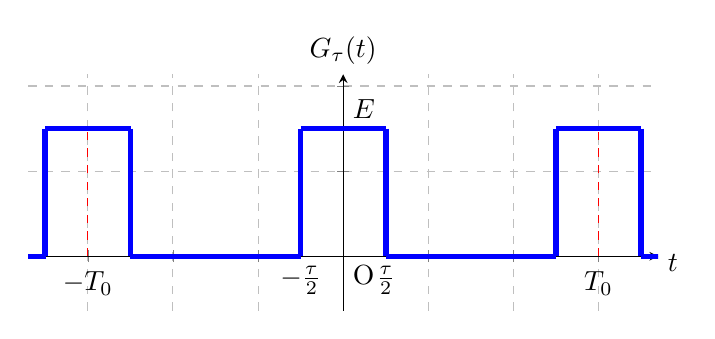
\begin{tikzpicture}
            \begin{axis}[
                axis lines = middle,
                xlabel = {$t$},
                xlabel style={at={(rel axis cs:1, 0.2)}, anchor=west},
                ylabel = {$G_{\tau}(t)$},
                ylabel style={at={(rel axis cs:0.5, 1)}, anchor=south},
                xmin = -3.7, xmax = 3.7,
                ymin = -0.2, ymax = 1.7,
                grid = major,
                grid style = dashed,
                scale only axis,
                width = 8cm,
                height = 3cm,
                axis equal,
                xtick = {-3, -2, -1, 0, 1, 2, 3},
                xticklabels = {$-T_0$, $ $, $ $, $ $, $ $, $ $, $T_0$},
                ytick = {0, 1, 2},
                yticklabels = {$ $, $ $, $ $},
            ]
            \addplot[domain=-3.7:-3.5, samples=100, smooth, line width=2pt, blue] {0};
            \addplot[smooth, line width=2pt, blue] coordinates {(-3.5, 0) (-3.5, 1.5)};
            \addplot[dashed, red] coordinates {(-3, 0) (-3, 1.5)};
            \addplot[domain=-3.5:-2.5, samples=100, smooth, line width=2pt, blue] {1.5};
            \addplot[smooth, line width=2pt, blue] coordinates {(-2.5, 1.5) (-2.5, 0)};
            \addplot[domain=-2.5:-0.5, samples=100, smooth, line width=2pt, blue] {0};
            \addplot[smooth, line width=2pt, blue] coordinates {(-0.5, 0) (-0.5, 1.5)};
            \addplot[domain=-0.5:0.5, samples=100, smooth, line width=2pt, blue] {1.5};
            \addplot[smooth, line width=2pt, blue] coordinates {(0.5, 1.5) (0.5, 0)};
            \addplot[domain=0.5:2.5, samples=100, smooth, line width=2pt, blue] {0};
            \addplot[smooth, line width=2pt, blue] coordinates {(2.5, 0) (2.5, 1.5)};
            \addplot[domain=2.5:3.5, samples=100, smooth, line width=2pt, blue] {1.5};
            \addplot[dashed, red] coordinates {(3, 0) (3, 1.5)};
            \addplot[smooth, line width=2pt, blue] coordinates {(3.5, 1.5) (3.5, 0)};
            \addplot[domain=3.5:3.7, samples=100, smooth, line width=2pt, blue] {0};
            \node at (axis cs:0, 0) [anchor=north west] {O};
            \node at (axis cs:0, 1.5) [anchor=south west] {$E$};
            \node at (axis cs:-0.5, 0) [anchor = north] {$-\frac{\tau}{2}$};
            \node at (axis cs:0.5, 0) [anchor = north] {$\frac{\tau}{2}$};
            \end{axis}
        \end{tikzpicture}
        \caption{周期矩形脉冲信号}
        \label{fig:periodic-rect-pulse-signal}
    \end{figure}

    则其在频域上的图像如图 \ref{fig:periodic-rect-pulse-signal-freq} 所示。
    \begin{figure}[H]
        \centering
        \begin{tikzpicture}
            \begin{axis}[
                axis lines = middle,
                xlabel = {$\omega$},
                ylabel = {$F_n$},
                ylabel style={at={(rel axis cs:0.5, 1)}, anchor=south},
                xmin = -10, xmax = 10,
                ymin = -0.3, ymax = 1.1,
                xtick = {-10, -8, -6, -4, -2, 0, 2, 4, 6, 8, 10},
                xticklabels = {$ $, $ $, $ $, $ $, $ $, $ $, $ $, $ $, $ $, $ $, $ $},
                ytick distance = 0.25,
                ytick = {-0.25, 0, 0.25, 0.5, 0.75, 1},
                yticklabels = {$ $, $ $, $ $, $ $, $ $, $\dfrac{E\tau}{T_0}$},
                grid = major,
                grid style = dashed,
            ]
            \addplot[dashed, domain=-10:10, samples=100, smooth, line width=2pt, blue] {sin(deg(x))/x};
            \draw[-stealth, smooth, line width=1pt, red] (axis cs:-8.3776, 0) -- (axis cs:-8.3776, 0.1034);
            \draw[-stealth, smooth, line width=1pt, red] (axis cs:-4.1888, 0) -- (axis cs:-4.1888, -0.2067);
            \draw[-stealth, smooth, line width=1pt, red] (axis cs:0, 0) -- (axis cs:0, 1);
            \draw[-stealth, smooth, line width=1pt, red] (axis cs:4.1888, 0) -- (axis cs:4.1888, -0.2067);
            \draw[-stealth, smooth, line width=1pt, red] (axis cs:8.3776, 0) -- (axis cs:8.3776, 0.1034);
            
            \node at (axis cs:0, 0) [anchor=north west] {O};
            \node at (axis cs:3.1416, 0) [anchor=north] {$\dfrac{2\pi}{\tau}$};
            \node at (axis cs:6.2832, 0) [anchor=north] {$\dfrac{4\pi}{\tau}$};
            \end{axis}
        \end{tikzpicture}
        \caption{周期矩形脉冲信号的频谱}
        \label{fig:periodic-rect-pulse-signal-freq}
    \end{figure}

    \begin{itemize}
        \item 谱线包络线为 $\sa$ 函数。
        \item 频谱谱线的间隔为 $\omega_0 = 2\pi / T_0$。
        \item 谱线包络线过零点位置为 $\omega_k = 2k\pi / \tau$,其中 $k \neq 0, k \in \set{Z}$。
    \end{itemize}
\end{example}

\begin{note}
    这里一般不考虑 $\omega_{-k}, k > 0$ 的情况。
\end{note}

\begin{theorem}
    周期为 $T_0$,脉冲宽度为 $\tau$,脉冲幅度为 $E$ 的周期矩形脉冲信号,谱线包络线则为
    \begin{align*}
        \frac{E\tau}{T_0}\sa{\left(\frac{\omega_0\tau}{2}\right)}.
    \end{align*}
\end{theorem}

\begin{proof}
    \begin{align*}
        F_n & = \frac{1}{T_0}\int_{-\tau/2}^{\tau/2}E\cdot \mathe^{-\mathi n\omega_0 t}\D{t} \\
        & = \frac{E}{T_0}\int_{-\tau/2}^{\tau/2}\mathe^{-\mathi n\omega_0 t}\D{t} \\
        & = \left.\frac{E}{T_0}\cdot\frac{1}{-\mathi n\omega_0}\cdot\left(\mathe^{-\mathi n\omega_0 t}\right)\right|_{-\tau/2}^{\tau/2} \\
        & = \frac{E}{T_0}\cdot\frac{1}{-\mathi n\omega_0}\cdot\left(\mathe^{-\mathi n\omega_0 \tau / 2} - \mathe^{\mathi n \omega_0\tau /2 }\right) \\
        & = \frac{E}{T_0}\cdot\frac{1}{-\mathi n\omega_0}\cdot\left(-2\mathi\sin\left(\frac{n\omega_0\tau}{2}\right)\right) \\
        & = \frac{E\tau}{T_0}\frac{\sin(n\omega_0\tau/2)}{n\omega_0\tau/2} \\
        & = \frac{E\tau}{T_0}\sa{\left(\frac{n\omega_0\tau}{2}\right)}.
    \end{align*}
\end{proof}

\begin{remark}
    非周期信号,在频率域上则为连续频谱;周期信号,在频率域上则为离散频谱。
    它们之间的转换关系,可以由下图 \ref{fig:periodic-nonperiodic-signal} 描述。
    \begin{figure}[H]
        \centering
        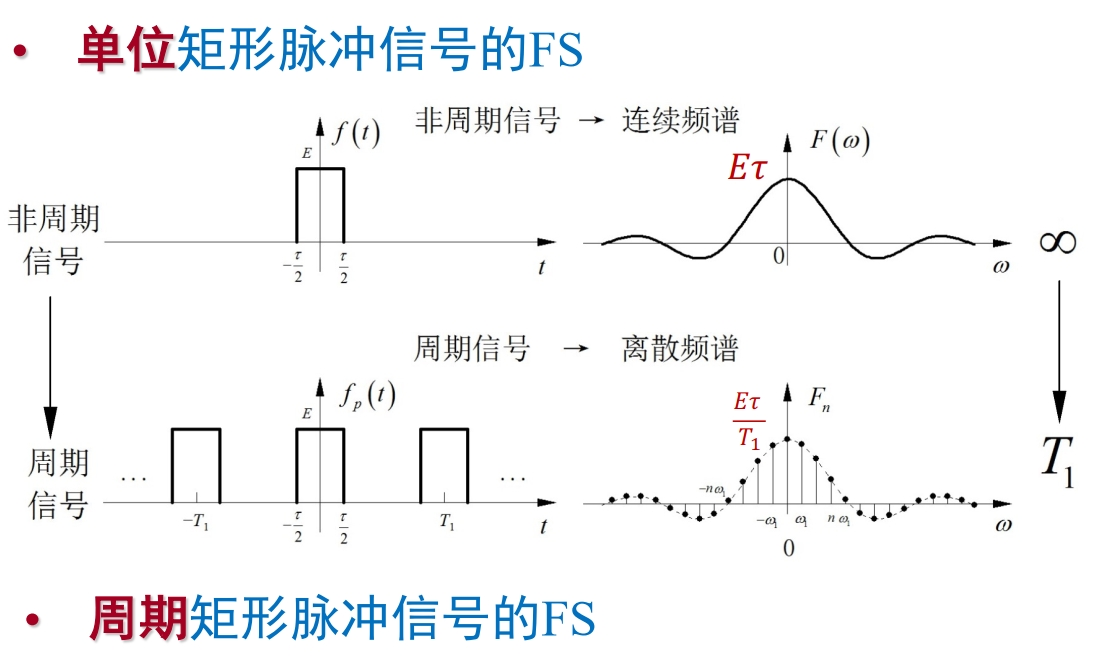
\includegraphics[width = 0.8\textwidth]{chap2/img/periodic-nonperiodic-signal.png}
        \caption{周期信号与非周期信号的频谱}
        \label{fig:periodic-nonperiodic-signal}
    \end{figure}
\end{remark}

\begin{property}[周期矩形脉冲信号的特点]
    在频域,能量主要集中在第一个零点以内!

    实际上,在允许一定失真的条件下,可以要求一个通信系统
    只把 $|\omega| \le 2\pi/\tau$ 频率范围内的各个频率分量传送过去,
    而舍弃 $|\omega| \ge 2\pi/\tau$ 的分量。

    常把 $-2\pi/\tau \le \omega \le 2\pi/\tau$ 这段频率范围成为矩形信号的\bd{频带宽度},
    简称\bd{带宽}。
    带宽只和脉冲的脉宽有关,而与脉高和周期均无关。
\end{property}

\begin{property}[周期信号的频谱谱线的特点]
    周期信号的频谱谱线的\bd{间隔}为
    \begin{align*}
        \omega_0 = \frac{2\pi}{T_0}.
    \end{align*}
    
    周期信号的频谱谱线的\bd{长度}为 $|F_n|$,其中
    \begin{align*}
        F_n = F(n\omega_0) = \frac{1}{T_0}\int_{t_0}^{t_0 + T_0}f(t)\mathe^{-\mathi n\omega_0 t}\D{t}.
    \end{align*}
\end{property}

\begin{note}
    由于复指数完备正交函数集中含有\bd{正负项},故周期矩形脉冲信号的谱线为\bd{双边谱}。
    对于 $n\omega_0$ 这一频率的频谱而言,频谱幅度为
    \begin{align*}
        |F_n| + |F_{-n}| = 2|F_n| = \frac{1}{2}\left(a_n^2 + b_n^2\right).
    \end{align*}
    一定要注意,它并不是 $|F_n|$。
\end{note}

\begin{exercise}
    已知 $f(t) = \sin t\cos 2t + 5\cos 3t \sin 4t$,求该函数的傅里叶级数。
\end{exercise}

\begin{solution}
    由三角函数的和差化积公式,有
    \begin{align*}
        f(t) & = \frac{1}{2}\left(\sin 3t - \sin t\right) + \frac{5}{2}\left(\sin 7t + \sin t\right) \\
        & = 2\sin t + \frac{1}{2}\sin 3t + \frac{5}{2}\sin 7t.
    \end{align*}
    此即为该函数的傅里叶级数。
\end{solution}
